\documentclass[main]{subfiles}

\begin{document}

\chapter{Código}
\label{chap:codigo}

El objetivo de esta sección es explicar como utilizar el código con el que vuela el cuadricóptero.

Para el entender en detalle que hace cada función, referirse a los comentarios en el código fuente.

El código se encuentre en el repositorio git, en la carpeta \verb+src/+. Todas las referencias a archivos en este anexo son respecto a la raíz del repositorio.Está pensado para compilarse y ejecutarse en un entorno linux. Si usás WINDOW\$ jodete. 

\section{Esquema general}
\label{sec:codigo:esquema-general}

\begin{wrapfigure}{r}{0.75\textwidth}
\vspace{-20pt}
\centering
  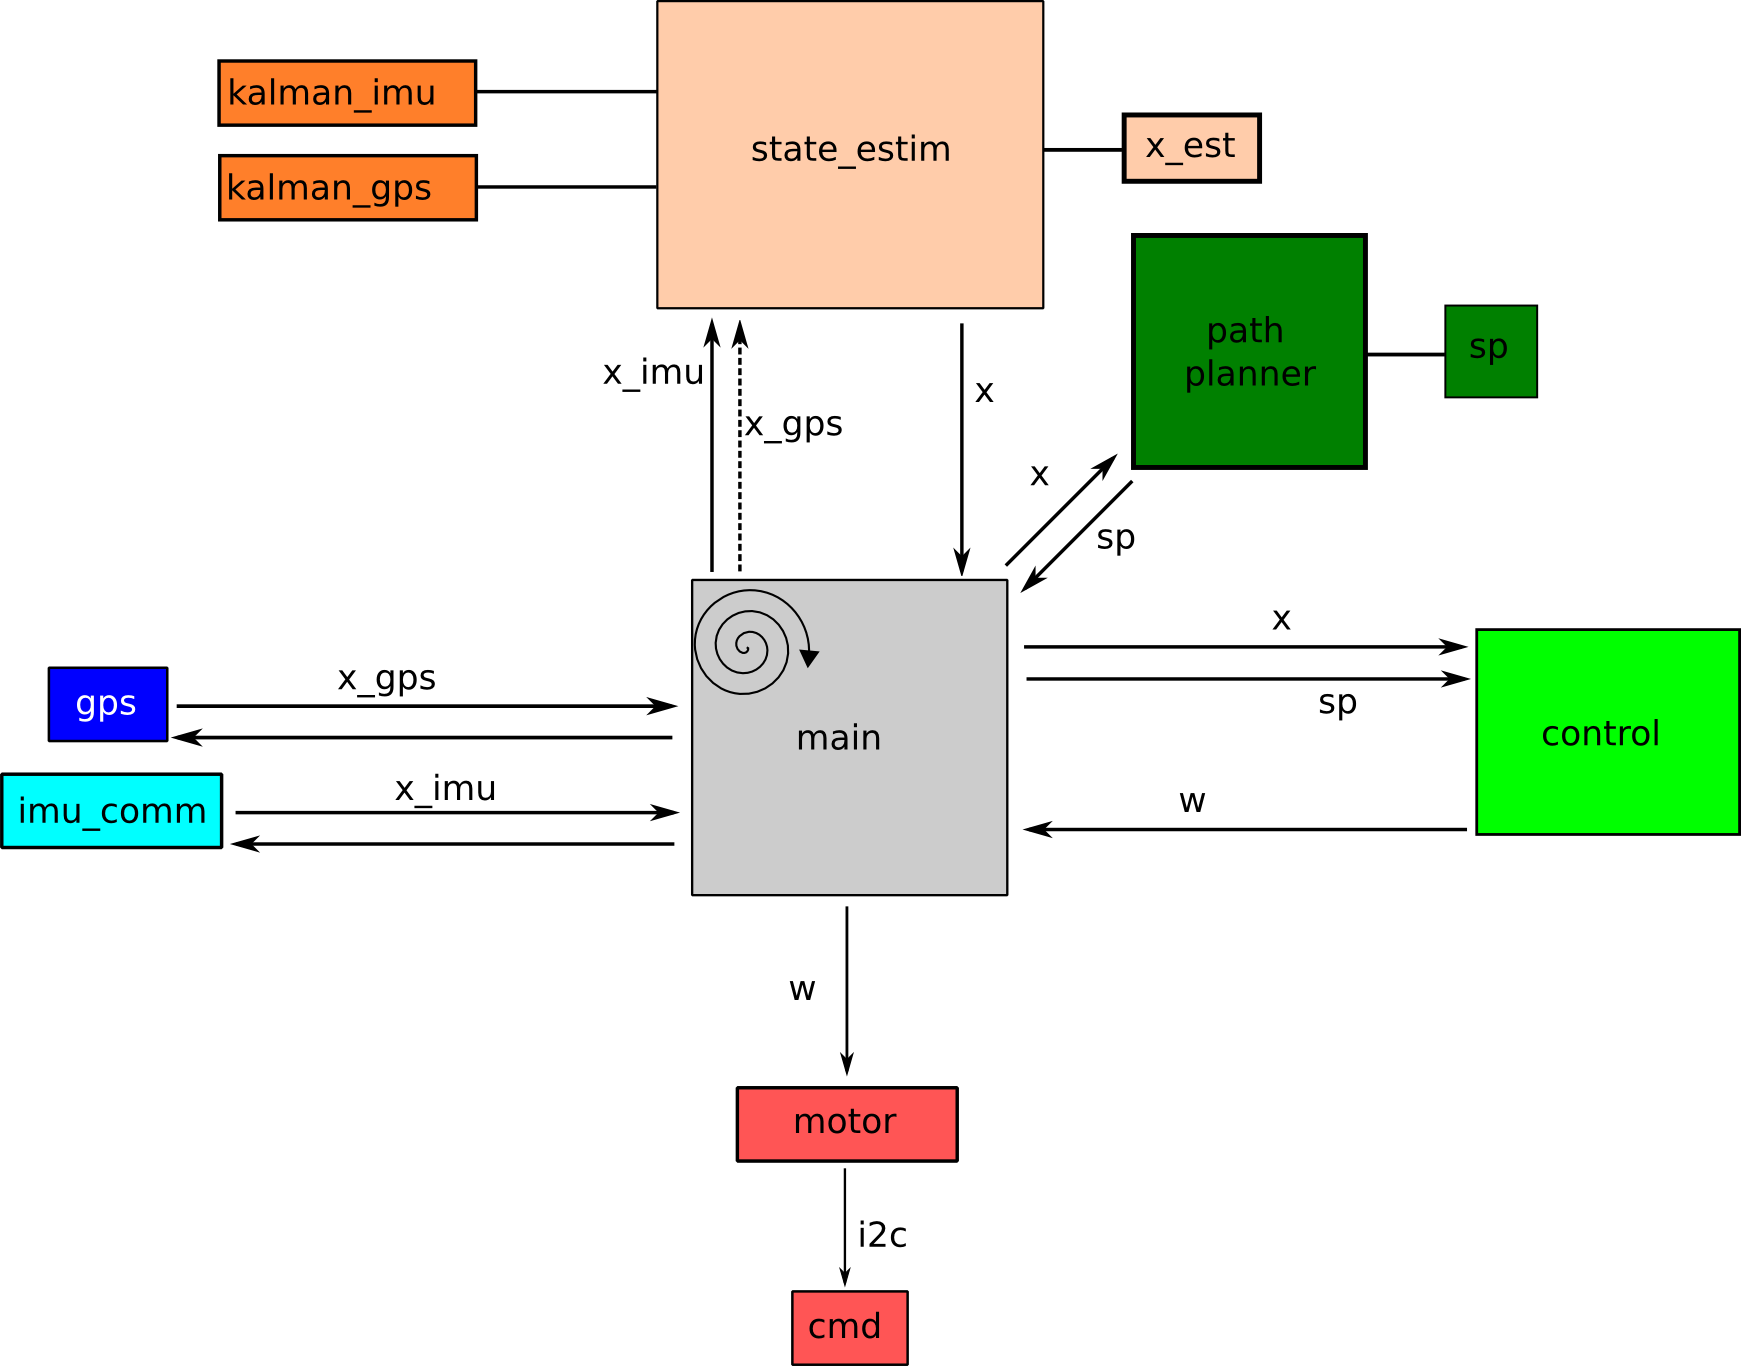
\includegraphics{./pics_codigo/code.png}
\caption{Estructura general del código.}
\vspace{-20pt}
\label{fig:codigo:code.png}
\end{wrapfigure}

El código tiene una estructura modular, está escrito en C, y cada bloque está implementado como una librería. La estructura general del código se resume en la figura \ref{fig:codigo:code.png}. Por claridad, no se muestran bloques intermedios, utilizados para intercomunicar las distintas partes.

Un loop normal, ejecutado por el programa principal (de ahora en más: \textit{main}) consiste en las siguiente etapas:
\begin{enumerate}
\item \textbf{imu:} Obtener una muestra nueva de la IMU, un datos nuevo de cada sensor.
\item \textbf{gps:} Si el GPS tiene una muestra lista, obtenerla.
\item \textbf{kalman:} Alimentar el filtro de Kalman con la información actualizada proveniente de los sensores.
\item \textbf{path planner:} Comparar el estado actual con el objetivo, y determinar si se completó el objetivo actual. En caso afirmativo, actualizar el estado objetivo a el siguiente en la lista.
\item \textbf{control:} Usando el estado actual y el estado deseado, determinar la acción de control a realizar.
\item \textbf{motor:} Actuar sobre los motores.
\end{enumerate}

Por información relativa a bloques, configuración, compilación, ejecución, etc, referirse a:
\begin{quote}
\begin{quote}
\begin{verbatim}
src/README
\end{verbatim}
\end{quote}
\end{quote}

% \subsection{\textit{imu\_comm}}
% \label{sec:codigo:imu_comm}

% La función de esta librería es hacer de interfaz con la IMU. Se encarga se presentar la información que la IMU envía mediante un puerto serie, armando una estructura con campos para cada sensor, timestamps, etc.

% Algunas funciones:
% \begin{itemize}
% \item \textbf{Calibración:} un conjunto de muestras que después se utilizan para estimar el offset de los giróscopos, y la altura inicial.
% \item \textbf{Conversión:} Cargando parámetros de calibración, convierte datos crudos provenientes de los sensores (bits) en datos útiles (aceleraciones, velocidades angulares, etc).
% \item \textbf{Ángulos de Euler:} Utilizando la información proveniente de acelerómetros y magnetómetro, calcula los tres ángulos de Euler.
% \item \textbf{Modo \textit{FAKE}:} Seteando \verb+IMU_COMM_FAKE+ a 1, la librería leerá de un log, en lugar de utilizar el puerto serie. Las características fundamentales del modo \textit{FAKE} son:
%   \begin{itemize}
%   \item Los tiempos no son un problema crítico, ya que no correrá en tiempo real.
%   \item La información en los logs está guardaba en \verb+ascii+ (la IMU trabaja en binario).
%   \end{itemize}
% \end{itemize}

% Archivos:
% \begin{quote}
% \begin{quote}
% \begin{verbatim}
% imu/imu_comm.[hc]
% test/imu_comm_test/imu_% comm_test.c
% % \end{verbatim}
% % \end{quote}
% % \end{quote}



% %TODO
% %descrip de c/u
% %macros para errores

% \section{Compilación}
% \label{sec:codigo:compilacion}

%TODO
% cross
% nativo

\subsection{Git}
\label{sec:codigo:git}

El código está almacenado en un repositorio git disponible en el DVD adjunto a esta documentación y en \textit{github}: \url{git://github.com/rlrosa/uquad.git}.

El repositorio ocupa aproximadamente 4GB, por lo que no conviene poner otras cosas en la tarjeta SD de la beagleboard, ya que sino se excederá de su capacidad.

\subsection{Comunicación}
\label{sec:codigo:comunicacion}

La forma básica de comunicarse con la beagleboard es mediante el puerto serie, usando un conversor \textit{RS2232} a USB. Durante el vuelo, la comunicación se establece mediante \textit{WiFi}, usando un dongle USB. El procedimiento para hacerlo funcionar es el siguiente:

\begin{enumerate}
\item Copiar el firmware \verb+scripts/rt73.bin+ a la beagleboard en \verb+/lib/firmware/+.
\item Instalar el software necesario haciendo \newline\verb+opkg install kernel-module-rt73usb rt73-firmware+.
\end{enumerate}

Una forma de conectarse es usando una red \textit{Ad-Hoc}. Para configurar la interfaz \verb+wlan0+\footnote{El dongle puede ser asociado a otra interfaz, como \textit{wlan1}, configurar la apropiada.} de para trabajar en modo \textit{Ad-Hoc} agregar las siguiente líneas a \verb+/etc/network/interfaces+:
\begin{quote}
\begin{quote}
\begin{verbatim}
auto wlan0
iface wlan0 inet static
address 10.42.43.2
netmask 255.255.255.0
wireless-mode ad-hoc
wireless-essid uquad
wireless-key s:uquaduquad123
\end{verbatim}
\end{quote}
\end{quote}

Luego, levantar una red en una laptop, en modo \textit{Ad-Hoc}, con nombre \textit{uquad} y contraseña \textit{uquaduquad123} en \textit{WEP 40/128-bit Key(Hex or ASCII)}.

La laptop tendrá la IP \textit{10.42.43.1}, y la beagleboard \textit{10.42.43.2}, por lo que se podrá hacer:
\begin{quote}
\begin{quote}
\begin{verbatim}
ssh root@10.42.43.2
\end{verbatim}
\end{quote}
\end{quote}

\subsubsection{Proxy}
\label{sec:codigo:proxy}

Para trabajar con la beagleboard en el laboratorio de medidas, es necesario configurar el proxy. Para ello, ejecutar los siguiente comandos en la beagleboard:
\begin{quote}
\begin{quote}
\begin{verbatim}
echo "option http_proxy http://httpproxy.fing.edu.uy:3128/" \
>> /etc/network/options.conf
echo "option http_proxy http://httpproxy.fing.edu.uy:3128/" \
>> /etc/opkg/arch.conf
\end{verbatim}
\end{quote}
\end{quote}

\subsubsection{ssh}
\label{sec:codigo:ssh}

La contraseña del usuario \textit{root} es apretar enter. Para evitar tener que hacerlo a menudo, por ejemplo si se trabaja remoto usando tramp+emacs, se puede agregar la clave pública de una laptop a la beagleboard, en\footnote{Crear el archivo y/o el directorio, si estos no existen.}.:
\begin{quote}
\begin{quote}
\begin{verbatim}
/home/root/.ssh/authorized_keys
\end{verbatim}
\end{quote}
\end{quote}

\subsubsection{ethernet}
\label{sec:codigo:ethernet}

La beagleboard sabe conectarse a una red en la que haya un servidor \textit{DHCP}. Elegirle un nombre en \verb+/etc/hostname+, por ejemplo \textit{beagle}, y luego hacer:
\begin{quote}
\begin{quote}
\begin{verbatim}
ssh root@beagle.local
\end{verbatim}
\end{quote}
\end{quote}

\subsection{Tiempos}
\label{sec:codigo:tiempos}

El \textit{main} corre sobre linux, lo cual simplifica algunas cosas, pero complica otras. Tener un sistema operativo en el medio puede introducir demoras inacceptables. No conviene ejecutar programas ni establecer conexiones (nuevas sesiones \textit{ssh}) mientras se ejecuta el rograma principal.

El acceso a memoria no volátil es lento, especialmente el acceso a la tarjeta \textit{micro-SD}. El \textit{main} guarda logs a una memora flash USB, en \verb+/media/sda1/+, ya que es significativamente más rápido. De cualquier forma, si se accede a memoria durante la ejecución del \textit{main}, \textbf{NO} será posible tener un loop estable, y por lo tanto \textbf{NO} se podrá volar el cuadricóptero. El \textit{main} crea, mediante \verb+fork()+, un \textit{logger} por cada log que se le pida, y dicho programa se encarga de pedir un bloque de RAM donde va almacenando información, y al finalizar el \textit{main} la guarda a memoria.

\subsection{Consideraciones de seguridad}
\label{sec:codigo:consideraciones-de-seguridad}

Al comenzar el \textit{main}, intentará establecer una conexión TCP con un servidor en la laptop, y abortará en caso de no tener éxito. Si en algún momento se pierde la conexión, por ejemplo por algún error en el driver del dongle \textit{WiFi}, el \textit{main} abortará, apagando los motores del cuadricóptero.

En caso de perderse ls conexión ssh, y que el cuadricóptero siga funcionando (porque la conexión TCP sigue funcionando), se puede detener el servidor que corre en la laptop, lo cual hará que el \textit{main} aborte y apague los motores.

NOTA: Cabe destacar que la performance del \textit{main} es \textbf{INACCEPTABLE} si se accede a memoria o si se abren sesiones ssh durante su ejecución.

\section{Salida - Logs}
\label{salidas-logs}

El \textit{main} genera varios logs durante su ejecución, que sirven determinar la causa de errores o comportamiento extraños durante un vuelo:
\begin{itemize}
\item Datos de la IMU - \textit{imu\_raw.log}
\item Datos utilizados para estimar el estado - \textit{kalman\_in.log}
\item Estado estimado - \textit{x\_hat.log}
\item Acción sobre el driver de los motores - \textit{w.log}
\end{itemize}

Referirse al código fuente por información sobre como habilitar logs, nombres, contenido, etc.

Cabe destacar que el espacio en RAM utilizado por el \textit{logger} es limitado, y dejará de guardar información una vez que se acabe.

\section{Debugging}
\label{sec:codigo:debugging}

Para probar el \textit{main} sin volar el cuadricóptero, puede resultar cómodo apagar el control de connectividad. Para ello, setear \verb+CHECK_NET_BYPASS+ a 1 en
\begin{quote}
\begin{quote}
\begin{verbatim}
src/common/uquad_config.h
\end{verbatim}
\end{quote}
\end{quote}

ADVERTENCIA: \textbf{NO} es recomendable hacer esto para una prueba con los motores prendidos, ya que la pérdida conexión implicaría la pérdida del control sobre el cuadricóptero.

\subsection{Ejecución a partir de un log}
\label{sec:codigo:ejecucion-a-partir-de-un-log}

Para debuggear el \textit{main}, se lo puede correr con un log conocido como entrada, lo cual permite analizar el efecto de cambios concretos. Para esto se debe configurar el módulo que lee de la IMU, avisándole que debe leer de un log. Esto se logra seteando \verb+IMU_COMM_FAKE+ a 1, en \verb+src/imu/imu_comm.h+.

\subsubsection{C Vs. MatLab}
\label{sec:codigo:c-vs-matlab}

Existe un script en \textit{MatLab} que reproduce el comportamiento del \textit{main}. Es muy útil para hacer pruebas y verificar el correcto funcionamiento del código en \verb+C+.

\begin{quote}
\begin{quote}
\begin{verbatim}
kalman/kalman_main.m
\end{verbatim}
\end{quote}
\end{quote}

Como argumento toma un log de datos crudos de la imu (\textit{imu\_raw.log}), como los generados por el \textit{main} o por \textit{imu\_comm\_test}:
\begin{quote}
\begin{quote}
\begin{verbatim}
src/test/imu_comm_test/imu_comm_test.c
\end{verbatim}
\end{quote}
\end{quote}

\section{Kernel}
\label{sec:codigo:kernel}

La beagleboard corre un linux, de la distribución:
\begin{itemize}
\item \url{http://www.angstrom-distribution.org/}
\end{itemize}
El kernel que viene por defecto es suficiente para \textit{casi} todo, hace falta configurar el puerto \textit{i2c-2} para que trabaje a 333kHz (en lugar de 400kHz).

Para compilar el kernel se utilizó \textit{Bitbake+OpenEmbedded}, y se lo cross-compiló desde Ubuntu 11.10 (64bits).

La versión del Kernel que se utilizó es la \textit{2.6.37}.

La información que se presenta a continuación se obtuvo de \cite{bib:oe-capture-changes}, \cite{bib:oe-angstrom-kernel-workflow} y del canal IRC \verb+#oe+.

\subsection{\textit{Cross-compiling - Bitbake+OpenEmbedded}}
\label{sec:codigo:cross-compiling-bitbake-oe}

Para poder compilar cosas para la beagleboard se puede usar un entorno de desarrollo como OpenEmbedded (de ahora en más \textit{OE}) y la herramienta para compilar, bitbake. bitbake es una suerte de make, pero en lugar de tratar con programas individuales, se maneja con recetas que listan programas y sus dependencias, y se encarga de compilar las cosas en el orden apropiado.

Todo lo que usa \textit{OE} se baja de internet mediante \textit{git}. A veces hay problemas con los servidores, y es cuestión de probar nuevamente en otro momento (o cambiar de servidor, revisar proxy, etc). Compilar una imagen entera, como para una SD, no es fácil, lleva tiempo y requiere que todos los servidores funcionen.

Para cross compilar en Ubuntu:
\begin{enumerate}
\item Ejecutar \verb+sudo dpkg-reconfigure dash+ y en el menu elegir la opción no. Por más información ver\newline\url{http://wiki.openembedded.org/index.php/OEandYourDistro}.
\item Descargar, configurar y actualizar el repositorio:
\begin{quote}
\begin{quote}
\begin{verbatim}
git clone git://git.angstrom-distribution.org/setup-scripts
cd startup-scripts
MACHINE=beagleboard ./oebb.sh config beagleboard
MACHINE=beagleboard ./oebb.sh update
source ~/.oe/environment-oecore
\end{verbatim}
\end{quote}
\end{quote}
\item Si se quisiera compilar ahora\footnote{Compilar la imagen lleva mucho tiempo, mejor configurar todo antes de compilar.}, hacer:
\begin{quote}
\begin{quote}
\begin{verbatim}
bitbake console-image
\end{verbatim}
\end{quote}
\end{quote}
\end{enumerate}

El script \verb+~/.oe/environment-oecore+ es responsable de generar variables que se utilizan durante la compilación. Cada vez que se abre una consola se cargan las variables globales y las declaradas en \verb+~/.bashrc+ (esto es independiente de compilar kernels, etc). Las variables en \verb+~/.oe/environment-oecore+ hay que cargarlas cada vez que se abre una nueva consola. Una de las cosas que hace el script es indicar la ruta al programa bitbake. Para verificar que el script fue correctamente ejecutado se puede escribir el comienzo del comando \verb+bit+ y apretar \textit{tab}, entre las opciones debería aparecer el comando bitbake.

Las recetas que utiliza bitbake (y nos interesan más) se encuentran en:
\begin{quote}
\begin{quote}
\begin{verbatim}
setup_scripts/sources/meta-ti/
\end{verbatim}
\end{quote}
\end{quote}
Algunos ejemplos:
\begin{itemize}
\item Configuración del kernel:
\begin{verbatim}
setup-scripts/sources/meta-ti/recipes-kernel/\
linux/linux-3.0/beagleboard/defconfig
\end{verbatim}
\item Receta para el kernel:
\begin{verbatim}
setup_scripts/sources/meta-ti/recipes-kernel/\
linux/linux-omap_3.0.bb
\end{verbatim}
\item Receta para el u-boot:
\begin{verbatim}
setup-scripts/sources/meta-ti/recipes-bsp/\
u-boot/u-boot_2011.12.bb
\end{verbatim}
\end{itemize}

Luego de haber incorporado las variables de \verb+~/.oe/environment-oecore+ ya no es necesario usar \verb+MACHINE=beagleboard ./oebb.sh+, se puede y debe usar directamente \textit{bitbake}.

Es recomendable hacer \verb+MACHINE=beagleboard ./oebb.sh update+ frecuentemente.
Algunos paquetes necesarios para poder compilar correctamente (pueden faltar otros):
\begin{verbatim}
sudo apt-get install\
   python-ply python-progressbar\
   texi2html cvs subversion gawk\
   chrpath texinfo diffstat
\end{verbatim}

\subsubsection{Como modificar el contenido de OE}
\label{sec:codigo:como-modificar-el-contenido-de-oe}

Para modificar un programa, como por ejemplo el \textit{u-boot}:
\begin{verbatim}
bitbake -c devshell u-boot
# se abre una consola en el dir temporal del u-boot
emacs board/ti/beagle/beagle.h
# editar, por ejemplo habilitar la UART2
git add board/ti/beagle/beagle.h
git commit -m 'uquad: habilitando UART2'
git format-patch HEAD~1
cp 001-uquad:-habilitando-UART2.patch $OE_BASE/
# incrementar la línea que dice "PR = "r4"", ponerle r5
bitbake u-boot
# buscar el resultado en setup-scripts/build/tmp*/deploy/images
\end{verbatim}

Para modificar el kernel y setear el \textit{i2c-2} a 333kHz:

\begin{verbatim}
bitbake -c devshell virtual/kernel
# se abre una cosola en el dir temporal del kernel
# ANTES de cambiar nada, hacer:
quilt new uquad-set-i2c-2-333kHz.patch
# Si se quiere hacer cambios en board-omap3beagle.c:
quilt add arch/arm/mach-omap2/board-omap3beagle.c
emacs arch/arm/mach-omap2/board-omap3beagle.c
# editar, por ejemplo setear i2c a 333kHz
# Ahora pedirle a quilt que arme un patch
quilt refresh
# El patch queda en patches/uquad-set-i2c-2-333kHz.patch
# Se copia a meta-ti/recipes-kernel/linux-3.0/
# Se edita meta-ti/recipes-kernel/linux_3.0.bb, agregando una línea antes de la q dice defconfig:
file://uquad-set-i2c-2-333kHz.patch;patch=1 \
# Ahora se compila haciendo
bitbake virtual/kernel
\end{verbatim}

\subsubsection{Comandos útiles - bitbake+OE}
\label{sec:codigo:comandos-bitbake-oe}

Algunos comando que pueden ser de utilidad:

\begin{itemize}
\item Para compilar un paquete individual, sin tomar en cuenta las dependencias:
\begin{verbatim}
bitbake -b receta.bb
\end{verbatim}
Ejemplo:
\begin{verbatim}
bitbake -b sources/meta-ti/recipes-bsp/u-boot/u-boot_2011.12.bb
\end{verbatim}
\item Para ver todas las recetas que se ejecutan como dependencias, hacer:
\begin{verbatim}
bitbake <receta> -g
\end{verbatim}
y luego mirar en \verb+task-depends.dot+.

Ejemplo:
\begin{verbatim}
bitbake console-base-image -g
\end{verbatim}
\item Para borrar todo lo compilado sobre un paquete, por ejemplo el u-boot, hacer:
\begin{verbatim}
bitbake -c clean u-boot
\end{verbatim}
\end{itemize}

\section{IMU}
\label{sec:codigo:imu}

%TODO
% arduino, ftdi, mongoose, etc

\section{Trabajo a futuro}
\label{sec:codigo:trabajo-a-futuro}

%TODO
% no esta implementado el path planner
% no anda bien lo de la matriz K en C, en realidad lo de la linealizacion (capaz es choto)

\end{document}